\section{Multivariate Densities Conditioned on Categorical Distributions}

\begin{figure}
  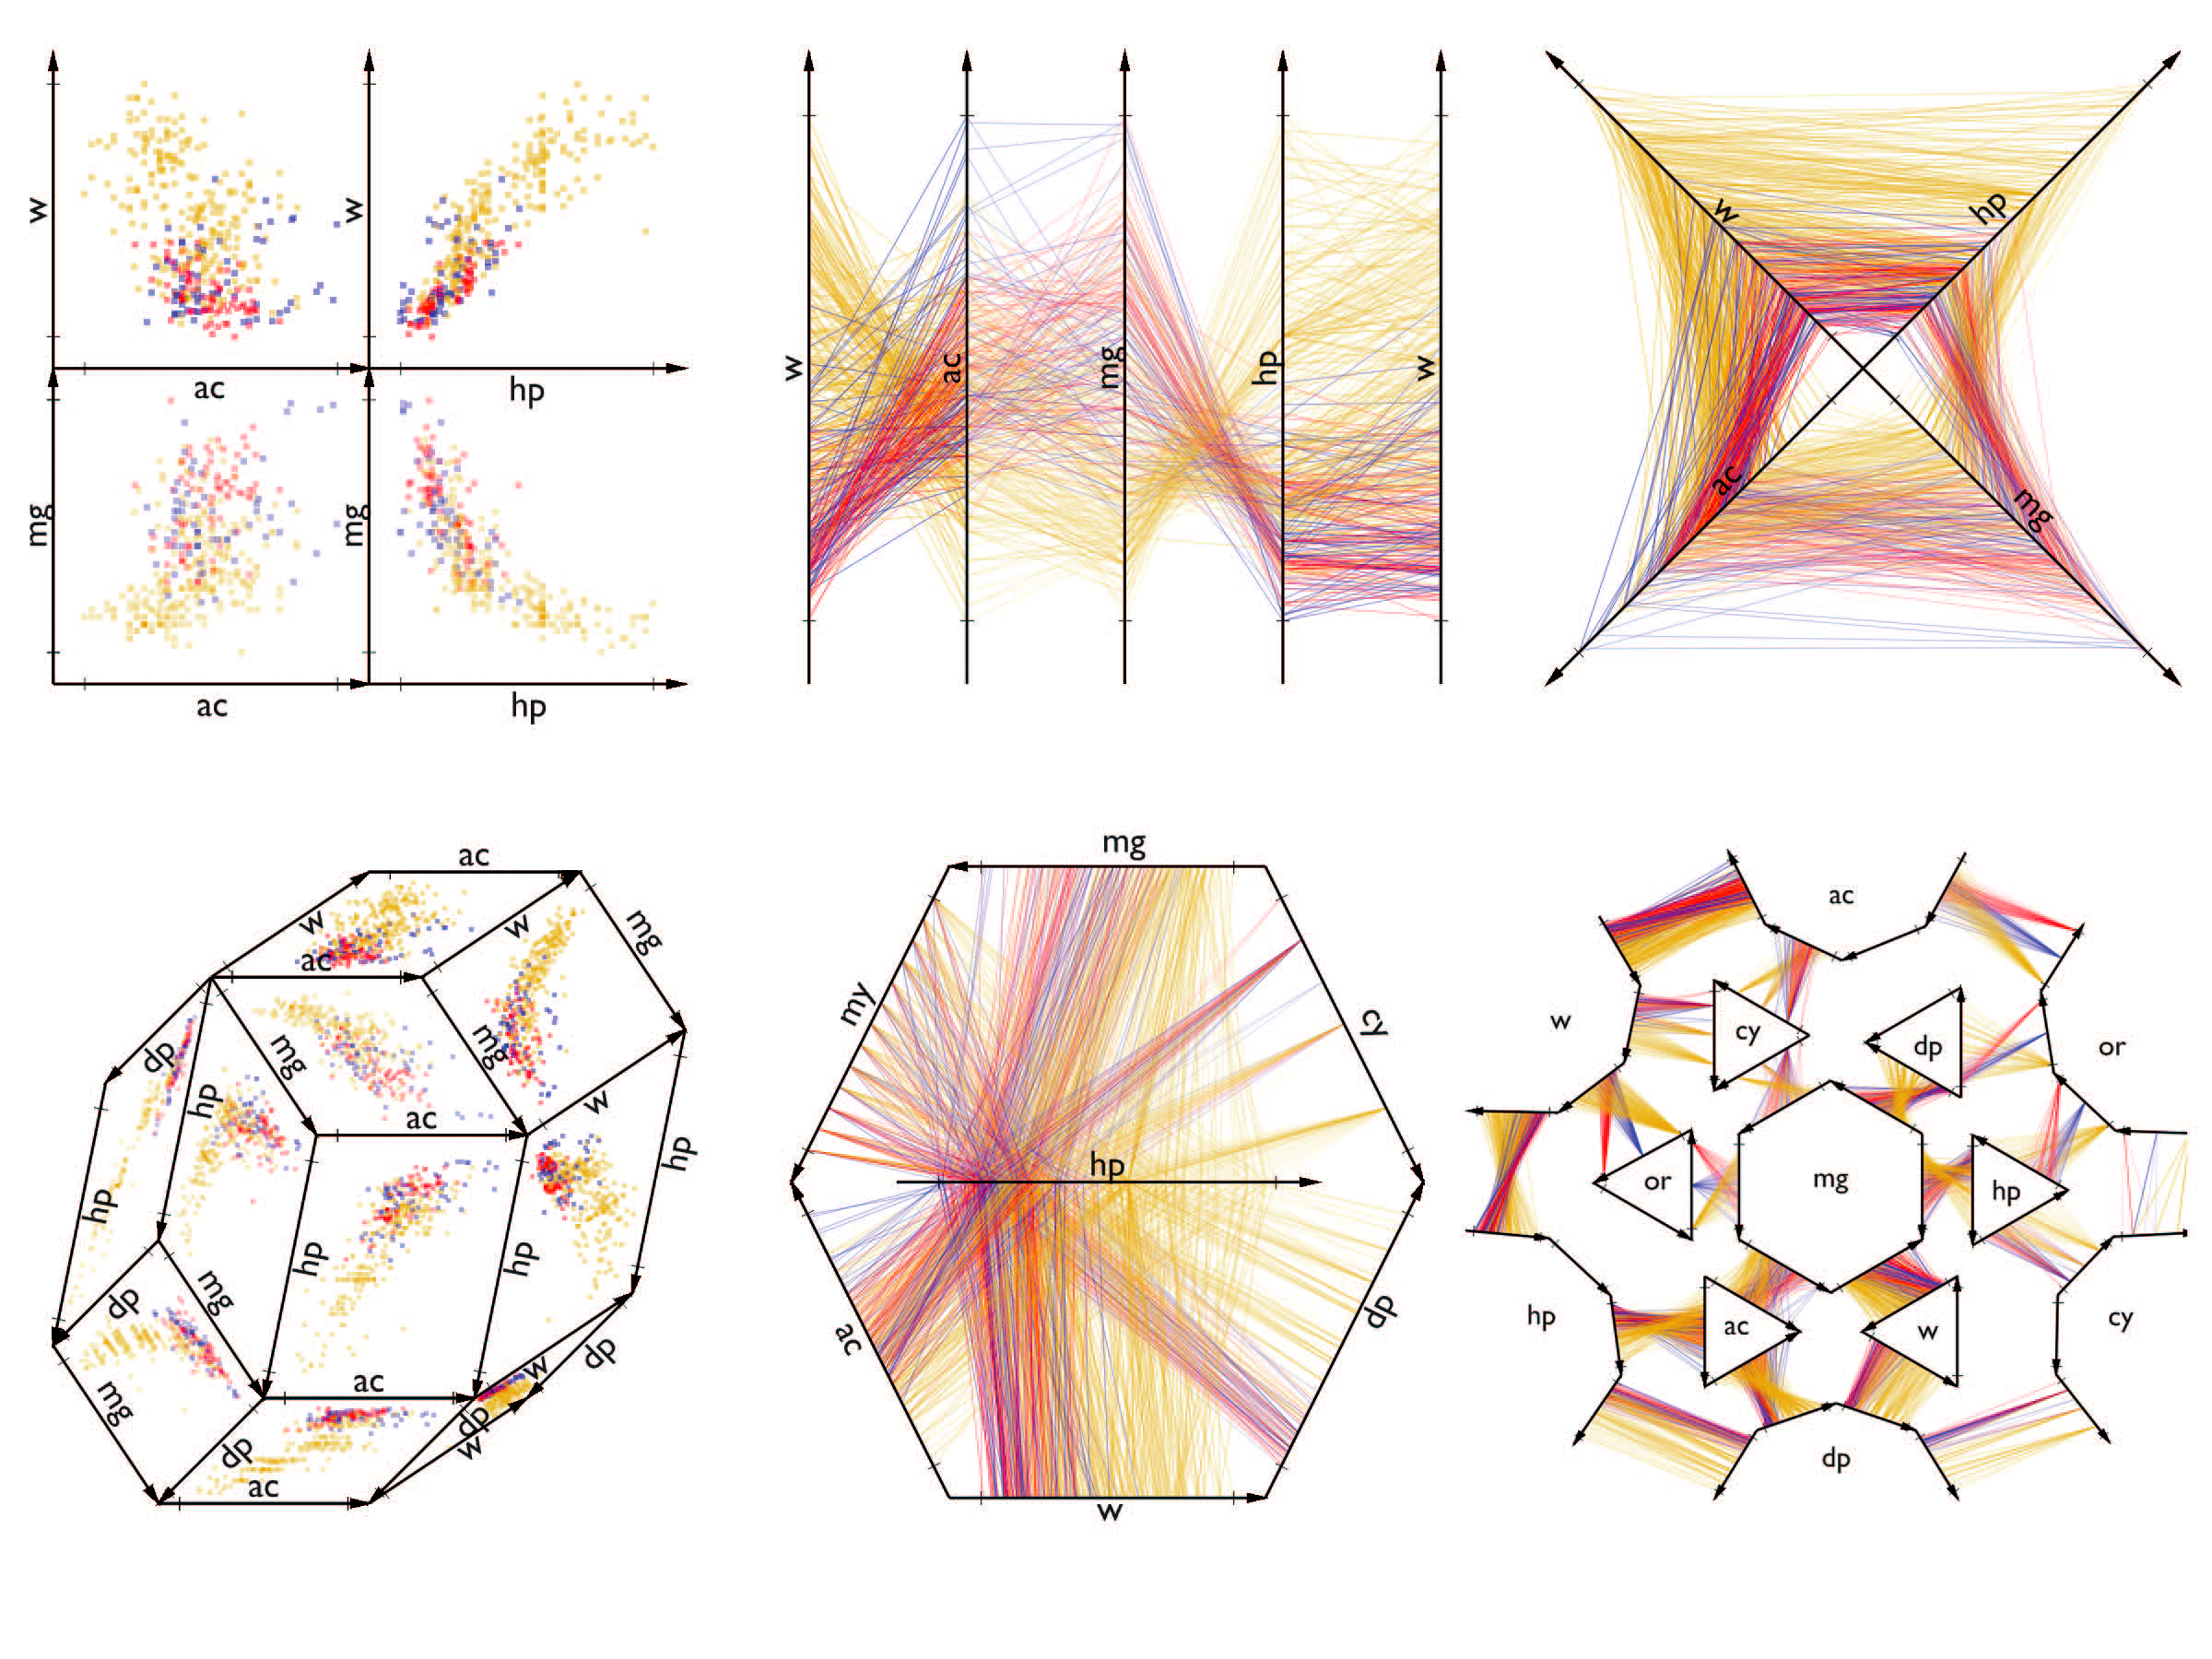
\includegraphics{flexaxis.png}
  \caption{Figure taken from \cite{claessen_van_wijk_2011} illustrates common
    methods for visualizing multivariate datasets.
  \label{fig:flexlink}
\end{figure}





There are a number of methods for showing how measurmeents of different
variables interact, and as showing figure~\ref{fig:flexlink} color is often
used to illustrate how these relationships are different for each category of
data. The colors can also change gradually to indicate changes in a quanitative
variable %%find citation for pca? with qualitative lines? but it's far less
%%ocmmon.
As seen in figure~\ref{fig:flexlink}, the common methods for showing
visualiztions are matrix of scatters \cite{matric of scatters paper}, parallel
coordinates \cite{islenberg, wegman}
